\chapter{Benchmark}
L'obiettivo dell'esercizio è quello di confrontare due sistemi con lo stesso sistema operativi, ma processori differenti, utilizzando il benchmark \textit{Nbody}. Esso simula l'evoluzione di N corpi celesti, sotto l'influenza della forza di gravità ed è molto utile per confrontare le prestazioni tra i due sistemi, dato che stressa:
\begin{itemize}
	\item \textbf{CPU}
	\item \textbf{Sottosistemi Floating-Point}
	\item \textbf{Chiamate ricorsive}
\end{itemize}
La complessità dell'algoritmo che lo implementa è un \textit{O($n^2$)}.
\\
Lo script \textit{launch\_nbody.sh} consente di avviare il benchmark al variare di N e del numero di ripetizioni impostate. Contestualmente ne raccoglie i tempi di esecuzione in millisecondi e li fornisce in output.

\section{Sistemi}
Il confronto è stato eseguito utilizzando due diverse architetture caratterizzate dai seguenti parametri:
\begin{table}[H]
	\begin{center}
		\begin{tabularx}{0.49\textwidth}{|c|X|}
			\hline
			\multicolumn{2}{|c|}{\textbf{Sistema 1}} \\
			\hline
			\textit{CPU} & Intel Core i7-7500U 7th Generation \\
			\hline
			\textit{Velocità di base} & 2.90 GHz \\
			\hline
			\textit{Cores} & 2 \\
			\hline
		\end{tabularx}
		\begin{tabularx}{0.49\textwidth}{|c|X|}
			\hline
			\multicolumn{2}{|c|}{\textbf{Sistema 2}} \\
			\hline
			\textit{CPU} & Intel Core i5-5700U 5th Generation \\
			\hline
			\textit{Velocità di base} & 2.20 GHz \\
			\hline
			\textit{Cores} & 2 \\
			\hline
		\end{tabularx}
	\end{center}
\end{table}

\section{Esecuzione}
Innanzitutto è stata fissata la dimensione \textit{N}, da passare come input al Benchmark necessaria per testare le performance dei due sistemi.
\\
Sono stati selezionati i seguenti 5 valori:
\begin{equation*}
	N = \begin{bmatrix}
		5.000 & 10.000 & 50.000 & 75.000 & 100.000
	\end{bmatrix}
\end{equation*}
Dopodichè, per ogni N, è stato estratto un \textbf{pre-campione} composto da 10 misurazioni tra di loro indipendenti (per garantirne l'indipendenza, il sistema è stato riavviato al termine di ogni misurazione).
\subsubsection{Dimensione Campionaria}
I pre-campioni sono risultati necessari per il calcolo della \textbf{dimensione campionaria n}, ovvero la dimensione effettiva di ogni campione che garantisce un prefissato errore E sulle medie.
\\
\begin{equation*}
	n = \left (\frac{t_{(\alpha/2,n-1)}*\sigma}{E}\right)
\end{equation*}
Considerando un intervallo di confidenza al \textit{95\%}, il parametro $\alpha$ sarà pari a \textit{0.05}, mentre avendo effettuato 10 misurazioni avremo un numero di gradi di libertà pari a 9.
\\
Il valore della distribuzione \textbf{T-student} viene dunque individuato a partire da questi due parametri.
\\
Per quanto riguarda l'errore \textit{E}, esso è stato ottenuto come percentuale sulla media dello specifico pre-campione. Nel nostro caso è stato previsto per ogni campione un errore del \textit{2.5\%}.
\\
Con il seguente script MATLAB è stato automatizzato il calcolo delle 5 dimensioni campionarie, memorizzate nel vettore \textit{vet\_n}:
\begin{minted}[framesep = 1mm,
	fontsize = \footnotesize,
	breaklines,
	]{MATLAB}
load precampione5000.txt;
load precampione10000.txt;
load precampione50000.txt;
load precampione75000.txt;
load precampione100000.txt;

N = 5;
vet_prc = [precampione5000,precampione10000,precampione50000,precampione75000,precampione100000];
%%
vet_media = zeros(1,N);
vet_sigma = zeros(1,N);
err = zeros(1,N);
vet_n = zeros(1,N);

t = abs(tinv(0.025,9));
for i=1:N
	vet_media(i) = mean(vet_prc(:,i)); 
	vet_sigma(i) = std(vet_prc(:,i));
	err(i) = vet_media(i)*0.025; 
	vet_n(i) = (t*vet_sigma(i)/err(i))^2;
end
\end{minted}
L'operazione è stata ripetuta su entrambi i sistemi, ottenendo le seguenti dimensioni campionarie:
\begin{equation*}
	n_{i7} = \begin{bmatrix}
		5 & 4 & 6 & 15 & 21
	\end{bmatrix}
\end{equation*}
\begin{equation*}
	n_{i5} = \begin{bmatrix}
		6 & 2 & 6 & 7 & 3
	\end{bmatrix}
\end{equation*}
Si è scelto, per ogni N, di tenere conto della stessa dimensione campionaria per i due sistemi ed in particolare della maggiore, in modo da garantire in ogni caso il minimo errore.
\begin{equation*}
	n = \begin{bmatrix}
		6 & 4 & 6 & 15 & 21
	\end{bmatrix}
\end{equation*}
Tale decisione è inoltre dettata dalla volontà di realizzare considerazioni statistiche operando sui vettori delle differenze tra i campioni, pertanto risulta necessario avere dimensioni coerenti.
\subsubsection{Prelievo dei Campioni}
Per garantire dati parametrici, sono state realizzate misurazioni indipendenti riavviando di volta in volta i sistemi.
\\ 
\\ Per \textbf{N = 5000}:
\begin{figure}[H]
	\centering
	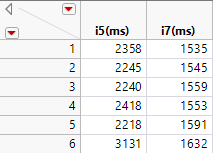
\includegraphics{img/hw0/5000.png}
	\caption{\textit{Campioni i5 e i7 per N=5000}}
\end{figure}
\begin{figure}[H]
	\centering
	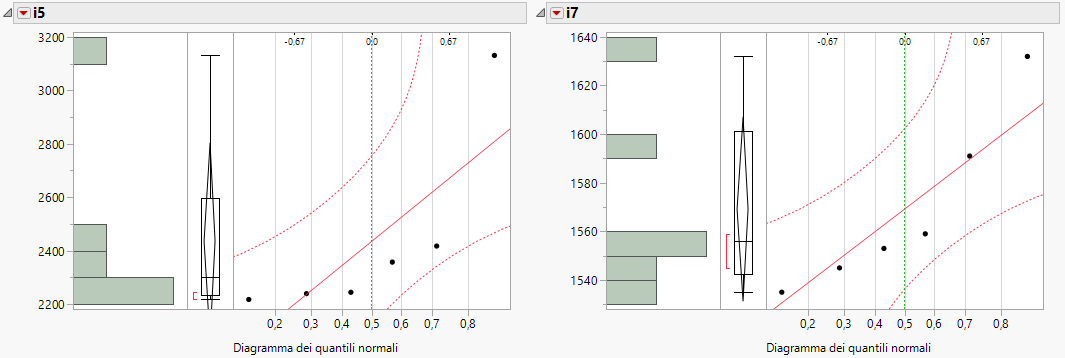
\includegraphics[width=1.1\textwidth]{img/hw0/5000distr.png}
	\caption{\textit{Distribuzione campioni i5 e i7 per N=5000}}
\end{figure}
\newpage
Per \textbf{N = 10000}:
\begin{figure}[H]
	\centering
	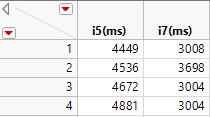
\includegraphics{img/hw0/10000.png}
	\caption{\textit{Campioni i5 e i7 per N=10000}}
\end{figure}
\begin{figure}[H]
	\centering
	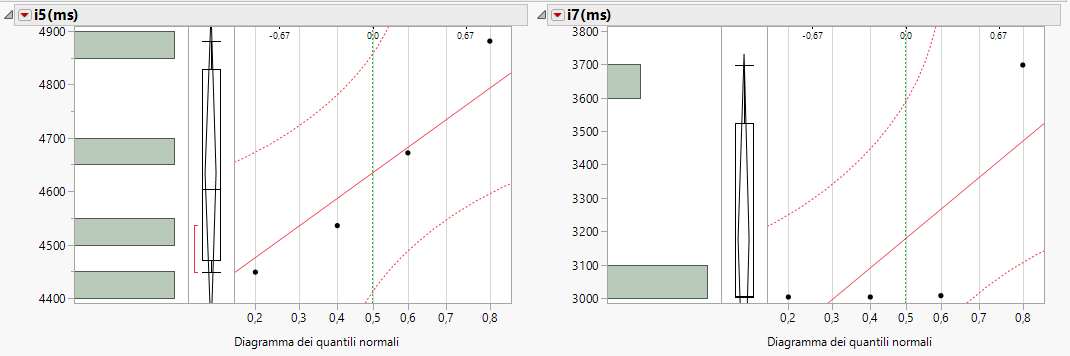
\includegraphics[width=0.9\textwidth]{img/hw0/10000distr.png}
	\caption{\textit{Distribuzione campioni i5 e i7 per N=10000}}
\end{figure}

Per \textbf{N = 50000}:
\begin{figure}[H]
	\centering
	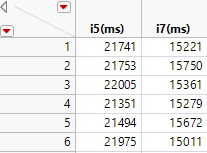
\includegraphics{img/hw0/50000.png}
	\caption{\textit{Campioni i5 e i7 per N=50000}}
\end{figure}
\begin{figure}[H]
	\centering
	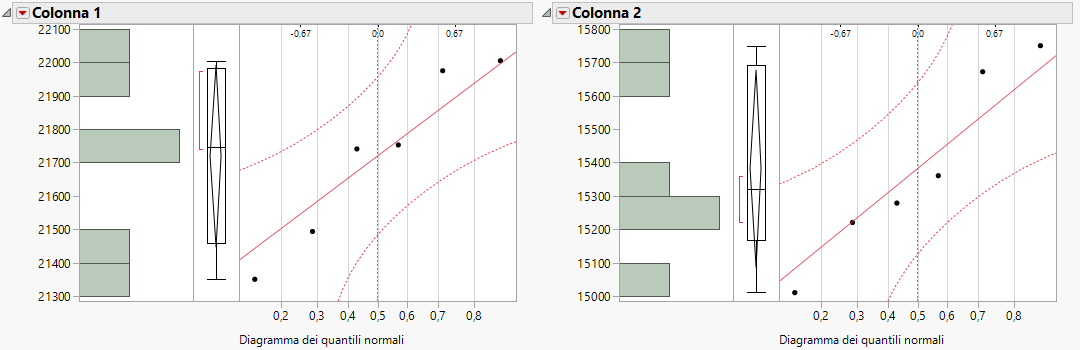
\includegraphics[width=0.9\textwidth]{img/hw0/50000distr.png}
	\caption{\textit{Distribuzione campioni i5 e i7 per N=50000}}
\end{figure}

Per \textbf{N = 75000}:
\begin{figure}[H]
	\centering
	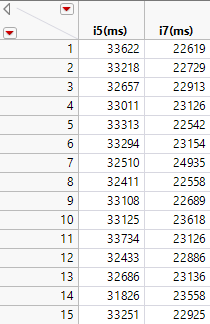
\includegraphics{img/hw0/75000.png}
	\caption{\textit{Campioni i5 e i7 per N=75000}}
\end{figure}
\begin{figure}[H]
	\centering
	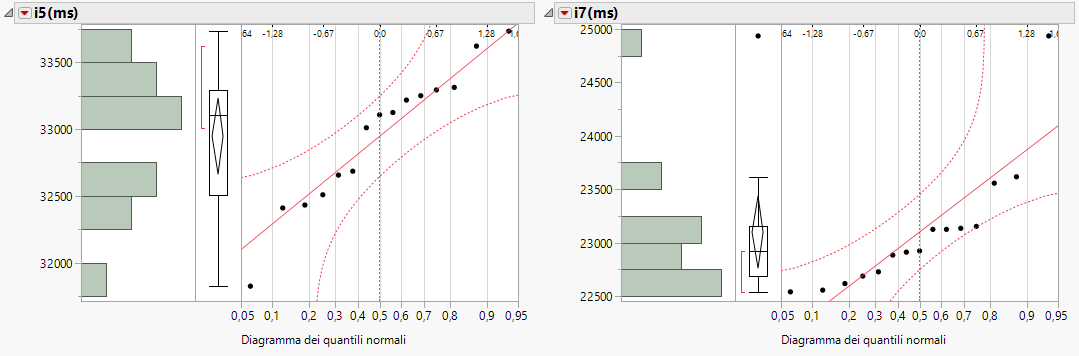
\includegraphics[width=1.1\textwidth]{img/hw0/75000distr.png}
	\caption{\textit{Distribuzione campioni i5 e i7 per N=75000}}
\end{figure}
\newpage
Per \textbf{N = 100000}:
\begin{figure}[H]
	\centering
	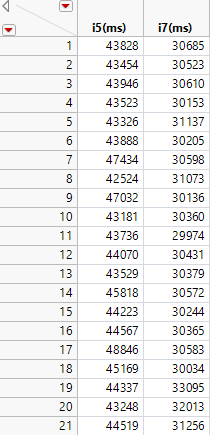
\includegraphics{img/hw0/100000distr.png}
	\caption{\textit{Campioni i5 e i7 per N=75000}}
\end{figure}
\begin{figure}[H]
	\centering
	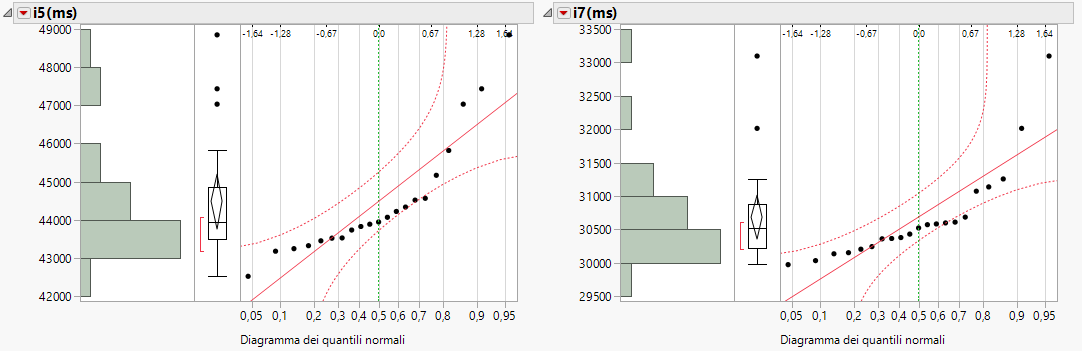
\includegraphics[width=0.9\textwidth]{img/hw0/100000.png}
	\caption{\textit{Distribuzione campioni i5 e i7 per N=100000}}
\end{figure}

Le distribuzioni risultanti sono tutte \textit{normali} eccetto quella per N = 100000. In ogni caso a noi interessa la normalità dei campioni differenza per potervi applicare lo \textit{Zero-Mean Test}.
\newpage
\subsubsection{Zero-Mean Test sui Campioni differenza}
Per ogni coppia di campioni è stato calcolato un vettore delle differenze. Su tutti i vettori delle differenze è stato applicato il test d'ipotesi \textit{Zero-Mean}. Esso non fa altro che testare la seguente ipotesi nulla:
\textit{$H_{0}$: i dati provengono da una distribuzione normale con media 0 e varianza sconosciuta.}
\\
Per poter applicare questo tipo di test, come già discusso in precendenza, dobbiamo dimostrare la normalità delle distribuzioni dei campioni eseguendo ancora una volta un \textit{quantile-quantile plot} tramite il tool JMP (tramite cui realizziamo anche il ttest).
\\
Analisi campione differenza per \textbf{N = 5000}:
\begin{figure}[H]
	\centering
	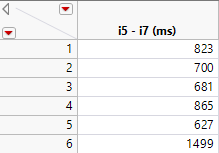
\includegraphics{img/hw0/diff1.png}
	\caption{\textit{Campione Differenza per N=5000}}
\end{figure}
\begin{figure}[H]
	\centering
	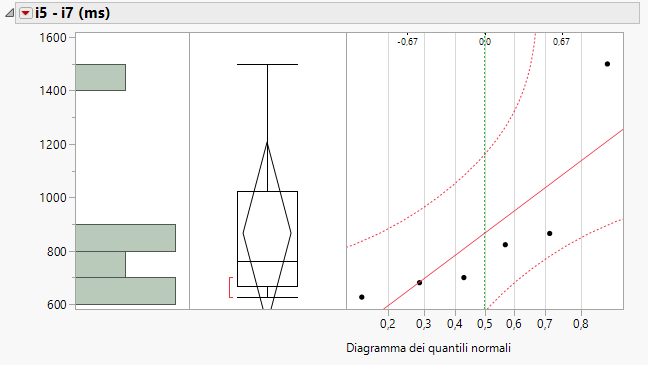
\includegraphics[width=0.9\textwidth]{img/hw0/statistiche5000_1.png}
	\caption{\textit{Distribuzione campioni Differenza per N=5000}}
\end{figure}
\begin{figure}[H]
	\centering
	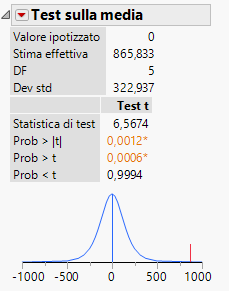
\includegraphics{img/hw0/test5000.png}
	\caption{\textit{Zero-Mean test per N=5000}}
\end{figure}

Analisi campione differenza per \textbf{N = 10000}:
\begin{figure}[H]
	\centering
	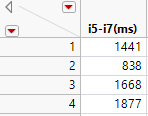
\includegraphics{img/hw0/diff2.png}
	\caption{\textit{Campione Differenza per N=10000}}
\end{figure}
\begin{figure}[H]
	\centering
	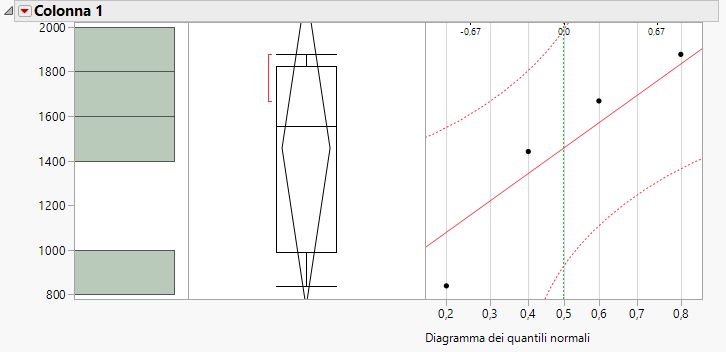
\includegraphics[width=0.9\textwidth]{img/hw0/statistiche10000.png}
	\caption{\textit{Distribuzione campioni Differenza per N=10000}}
\end{figure}
\begin{figure}[H]
	\centering
	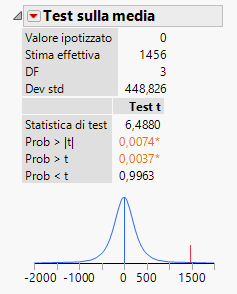
\includegraphics{img/hw0/test10000.png}
	\caption{\textit{Zero-Mean test per N=10000}}
\end{figure}

Analisi campione differenza per \textbf{N = 50000}:
\begin{figure}[H]
	\centering
	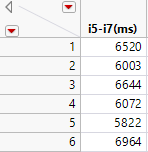
\includegraphics{img/hw0/diff3.png}
	\caption{\textit{Campione Differenza per N=50000}}
\end{figure}
\begin{figure}[H]
	\centering
	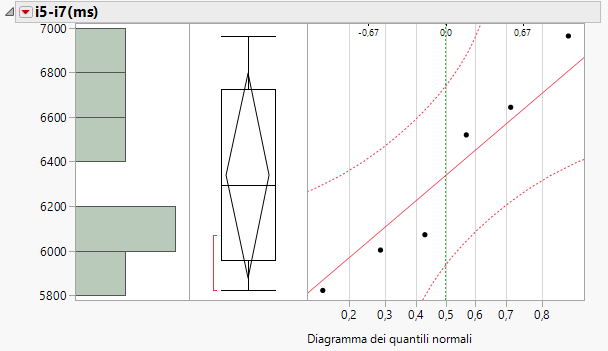
\includegraphics[width=0.9\textwidth]{img/hw0/statistiche50000.png}
	\caption{\textit{Distribuzione campioni Differenza per N=50000}}
\end{figure}
\begin{figure}[H]
	\centering
	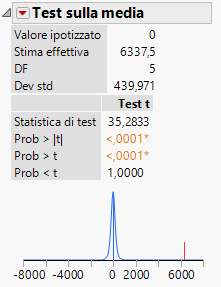
\includegraphics{img/hw0/test50000.png}
	\caption{\textit{Zero-Mean test per N=50000}}
\end{figure}

Analisi campione differenza per \textbf{N = 75000}:
\begin{figure}[H]
	\centering
	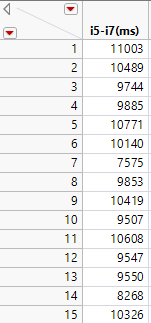
\includegraphics{img/hw0/diff4.png}
	\caption{\textit{Campione Differenza per N=75000}}
\end{figure}
\begin{figure}[H]
	\centering
	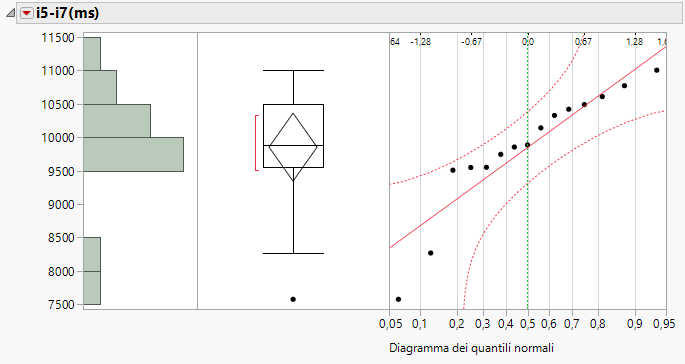
\includegraphics[width=0.9\textwidth]{img/hw0/statistiche75000.png}
	\caption{\textit{Distribuzione campioni Differenza per N=75000}}
\end{figure}
\begin{figure}[H]
	\centering
	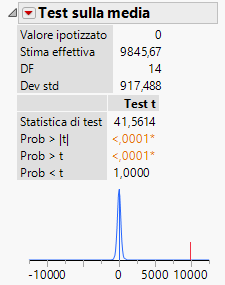
\includegraphics{img/hw0/test75000.png}
	\caption{\textit{Zero-Mean test per N=75000}}
\end{figure}

Analisi campione differenza per \textbf{N = 100000}:
\begin{figure}[H]
	\centering
	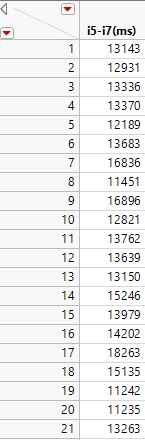
\includegraphics{img/hw0/diff5.png}
	\caption{\textit{Campione Differenza per N=100000}}
\end{figure}
\begin{figure}[H]
	\centering
	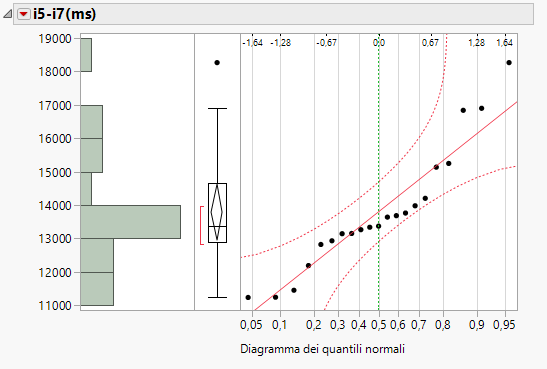
\includegraphics[width=0.9\textwidth]{img/hw0/statistiche100000.png}
	\caption{\textit{Distribuzione campioni Differenza per N=100000}}
\end{figure}
\begin{figure}[H]
	\centering
	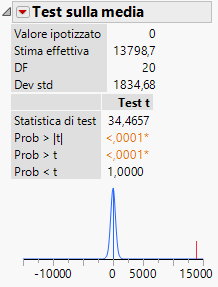
\includegraphics{img/hw0/test100000.png}
	\caption{\textit{Zero-Mean test per N=100000}}
\end{figure}
La normalità è stata dimostrata per ognuno dei 5 campioni differenza, pertanto è stato possibile applicare il test parametrico, il quale in tutti i casi ha scartato l'ipotesi nulla a favore di quella alternativa.
\\
Il test ha permesso di scartare l'ipotesi nulla con una significatività del 5\%, dunque le distribuzioni non hanno media nulla.
\\
Ciò dimostra che i due sistemi, sottoposti allo stesso benchmark, hanno fornito, al variare di N, risposte statisticamente differenti.  